\documentclass{article}
\usepackage{tikz}

\begin{document}

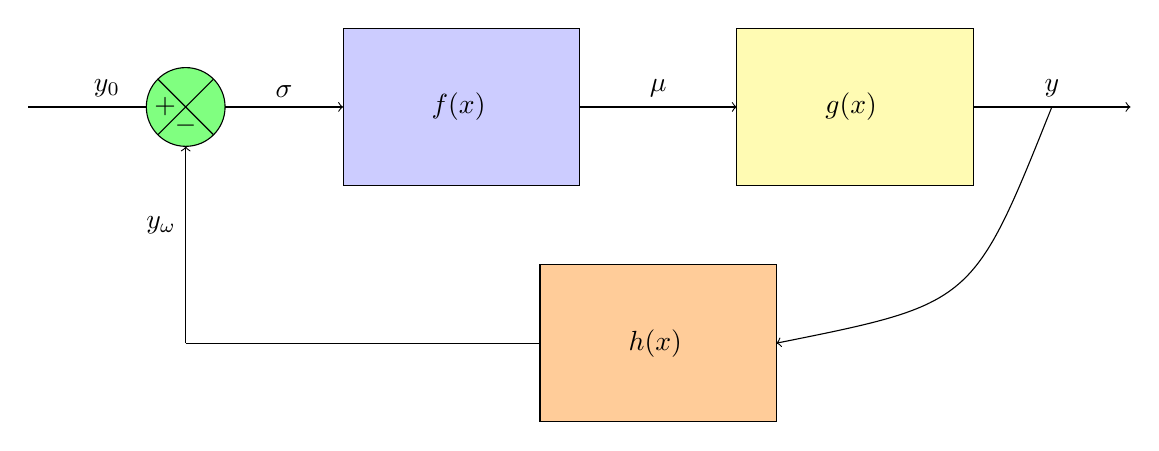
\begin{tikzpicture}
    \draw[fill=green!50] (0,0) circle (0.5 cm);
    \draw (-2,0) -- (-0.5,0);
    \draw (-1,0) node[anchor=south] {$y_0$};
    \draw (-0.35,0.35) -- (0.35,-0.35);
    \draw (0.35,0.35) -- (-0.35,-0.35);
    \draw (0,0) node[anchor=east] {$+$};
    \draw (0,0) node[anchor=north] {$-$};
    \draw [->](0,-3) -- (0,-0.5);
    \draw (0,-1.5) node[anchor=east] {$y_\omega$};
    \draw (0,-3) -- (4.5,-3);
    \draw [fill=orange!40] (4.5,-4) rectangle (7.5,-2);
    \draw (5.5,-3) node[anchor=west] {$h(x)$};
    \draw [->](0.5,0) -- (2,0);
    \draw (1.25,0) node[anchor=south] {$\sigma$};
    \draw [fill=blue!20] (2,-1) rectangle (5,1);
    \draw (3,0) node[anchor=west] {$f(x)$};
    \draw [->](5,0) -- (7,0);
    \draw (6,0) node[anchor=south] {$\mu$};
    \draw [fill=yellow!30] (7,-1) rectangle (10,1);
    \draw (8,0) node[anchor=west] {$g(x)$};
    \draw  [->] (10,0) -- (12,0);
    \draw (11,0) node[anchor=south] {$y$};
    \draw [->](11,0) .. controls (10,-2.5) .. (7.5,-3);
\end{tikzpicture}

\end{document}